\usepackage{shared/cs45}

\title{CS 45, Lecture 6}
\subtitle{Command Line Environment}
\date{Winter 2023}
\author{Akshay Srivatsan, Ayelet Drazen, Jonathan Kula}

\newcommand{\var}[1]{\texttt{\$#1}}
\newcommand{\cmd}[1]{\mintinline{shell}{#1}}

\begin{document}

\maketitle

\frame{\titlepage}

\begin{frame}
  \frametitle{Outline}
  \tableofcontents[hidesubsections]
\end{frame}

\begin{frame}{Announcements}
  \begin{itemize}
    \item Assignment 2 is due today; let us know if you need an extension
      (beyond the usual late days).
    \item Assignment 3 will be coming out later today.
  \end{itemize}
\end{frame}


\section{Review}

\begin{frame}{Text Editors}
  In the previous lecture, we saw:
  \begin{itemize}
    \item
      How to edit files in the terminal
      \pause
    \item
      How to enter/exit a full screen program
      \pause
  \end{itemize}
  In this lecture, we will see:
  \begin{itemize}
    \item
      How to configure and customize your shell
      \pause
    \item
      How to multitask in the terminal
      \pause
    \item
      How to run multiple programs side-by-side
  \end{itemize}
\end{frame}

Before we get into that, there are a few similar terms that are often confused;
let's get into what they mean and how they're different.

\begin{frame}{Terminal vs. Shell vs. Command Line}
  \begin{definition}[terminal]
    The \textsc{terminal} is the window you open.  Think of it like a web
    browser.
  \end{definition}

  \pause

  \begin{definition}[shell]
    The \textsc{shell} is the program you use to launch other programs.
    Think of it like \href{https://google.com}{Google}.
  \end{definition}

  \pause

  \begin{definition}[cli]
    A \textsc{command line interface (CLI)} is a generic term for a text-based program which runs
    within a terminal.  Think of this like \enquote{the web}.  A \textsc{CLI
    program} or a \textsc{TUI program} is like a website.
  \end{definition}
\end{frame}

\section{The Environment}

We've already seen how you can control the behavior of CLI programs using
flags, but there's another way to configure them.  Each program runs in what's
called an \enquote{environment}.

\begin{frame}{Contents of the Environment}
  The \enquote{environment} a program runs in includes several things:
  \pause
  \begin{itemize}
    \item
      The user who's running it\pause
    \item
      The files on the filesystem\pause
    \item
      Environment variables (configuration variables)\pause
    \item
      \texttt{stdin} and \texttt{stdout} (and \texttt{stderr}), which we've already seen
  \end{itemize}
\end{frame}

Each of these affects running programs in different ways.  Some of them control
what a program can or cannot do, others control the default behavior of
programs.

\subsection{Configuration}

\begin{frame}{Input/Output}
  We already saw this in Lecture 2, but we can control the default input and
  output files of a program using \textsc{redirection}, i.e., the \texttt{<},
  \texttt{>}, \texttt{>>}, and \texttt{|} operators.

  \pause

  By default, input comes from the terminal (\texttt{/dev/tty*} or
  \texttt{/dev/pts/*}); you can see the name of the \enquote{controlling
  terminal} of a program by running \cmd{tty}.

  \mode<article> {
    A \textsc{controlling terminal} is essentially which terminal window a
    program is running in.
  }

  \pause

  Input and output can be redirected, but a program is bound to a specific
  window.  When that window is closed, the program will exit.
\end{frame}

\begin{frame}[fragile]{Environment Variables}

  \textsc{Environment variables} are a way to configure a program's default
  behavior.

  \pause

  We've already seen shell scripting variables, environment variables are
  basically the same thing except they're \enquote{exported} so other programs
  can use them.

  \pause

  For example, the \var{PATH} variable determines where programs can be
  located.  If a program isn't found \enquote{on your \var{PATH}}, you'll
  get a \enquote{command not found} error.

  \pause

  Other common variables:
  \begin{description}
    \item[\var{TERM}:] Which terminal you're using.
    \item[\var{USER}:] Your username
    \item[\var{EDITOR}:] Which editor you prefer
    \item[\var{PWD}:] Your current directory
  \end{description}

\end{frame}

\begin{frame}[fragile]{PATH}
  My \var{PATH} looks like this:
  \begin{minted}{text}
/home/akshay/.local/bin:/usr/local/bin:/usr/bin:/usr/local/sbin:
/var/lib/flatpak/exports/bin:/usr/bin/site_perl:
/usr/bin/vendor_perl:/usr/bin/core_perl
  \end{minted}

  This is a list of directories, where each directory is separated by colons
  (\cmd{:}).

  When you run a program like \cmd{grep}, the shell looks in each directory on
  your \var{PATH} from left to right.
\end{frame}

\begin{frame}[fragile]{Setting Environment Variables}
  You can \enquote{export} an environment variable as follows:
  \begin{minted}{shell}
    export MYVAR="hi"
    python -c 'import os; print(os.getenv("MYVAR"))'
  \end{minted}

  \mode<article> {
    Note that even though I ran a Python program, not a shell program, it was
    able to read the value of \var{MYVAR}.
  }

  \mode<article> {
    We saw this on Part 2 of Assignment 2 when we exported \var{SUNET} to be
    your SUNet ID.
  }

  \pause

  You can temporarily set an environment variable as follows:
  \begin{minted}{shell}
    MYVAR=hi python -c 'import os; print(os.getenv("MYVAR"))'
  \end{minted}

  \mode<article> {
    In this case, only that one line gets run with \var{MYVAR} set to
    \enquote{hi}; after that, \var{MYVAR} goes back to its old value (or
    becomes undefined).
  }
\end{frame}

Environment variables are ubiquitous in UNIX, and pretty much every programming
language has a way to read and write them.  The shell makes it incredibly easy by
treating them as normal variables; in other languages, you'd have to call a
function to get or set them.

By default, environment variables only persist until you exit the shell (or
close the terminal window).  We'll see later how to make them persist.

\subsection{Permissions}

\begin{frame}[fragile]{Users and Groups}
  We also talked about this a bit in Lecture 2, but every command you run runs
  as a specific user.

  \pause

  The variable \var{USER} holds your username (although this is just a
  convention, there's no actual requirement that the contents match).

  \pause

  Every user may belong to one or more \enquote{groups}, which you can see by
  running \cmd{groups}.

  For example, I'm in the groups:
  \begin{minted}{shell}
 % groups
docker uucp audio wheel akshay
  \end{minted}

  \mode<article> {
    Each of these groups gives me special permissions and abilities.  For
    example:

    \begin{itemize}
      \item The group \enquote{docker} means I can run the program
        \enquote{Docker} (which usually only root can run) without using
        \texttt{sudo}.
      \item The group \enquote{uucp} means I can read and write to
        serial ports (the name is a holdover from the old \enquote{unix-to-unix
        copy} program).
      \item The group \enquote{audio} means I can use my computer's
        speakers (you wouldn't have these permissions on a remote server like \texttt{myth}, for example).
      \item The group \enquote{wheel} gives me permission to use the program
        \texttt{sudo}.  Trying to use \texttt{sudo} without this permission
        will cause an error.
      \item The group \enquote{akshay} gives me permission to\textellipsis{}
        access my own files?  This is kind of useless nowadays (I can
        \textit{always} access my own files, since I own them), but it used to
        be used as a way to share files among different users on the same
        computer.
    \end{itemize}

    Historically, groups were used to share files among different users on a
    multi-user system (like \textit{myth}).  For example, Professor Engler's
    research group might have had a corresponding UNIX group named
    \texttt{engler\_group}, so we could all collaborate on files and source
    code.  Nowadays this has been replaced with other means of collaboration
    like \cmd{git}, and everyone has their own laptop, so this use has become
    more rare.
  }
\end{frame}

\begin{frame}[c]{Permissions}
  On UNIX, you must have the appropriate \enquote{permissions} to do certain
  actions.

  \pause

  \begin{center}
    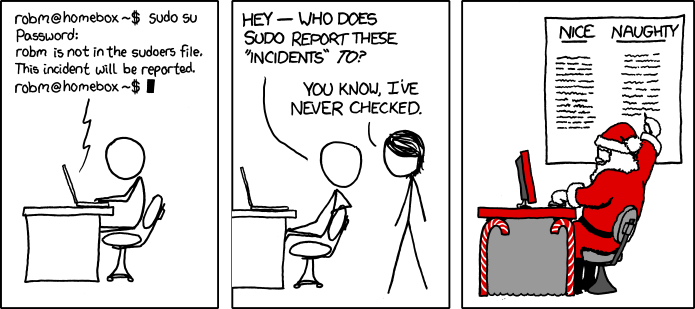
\includegraphics[width=0.7\paperwidth]{images/incident.png}
  \end{center}

  Source: \href{https://xkcd.com/838/}{xkcd 838}
\end{frame}

One of the most important types of permissions (and probably the only one
you'll see frequently) is permissions on specific files.

\begin{frame}{File Permissions}
  Every file has an \enquote{owner} and a \enquote{group}.
  \pause

  Every file has three sets of permissions: owner permissions, group
  permissions, and everyone else permissions.
  \pause

  \texttt{r} means \enquote{permission to read}, \texttt{w} means
  \enquote{permission to write}, and \texttt{x} means \enquote{permission to
  execute (i.e., run)}.
  \pause

  You can see file permissions by running \cmd{ls -l}.
\end{frame}

\begin{frame}[fragile]{File Permissions Example}{Output of \texttt{ls}}
  \begin{minted}{shell}
-rwxr-xr-x 1 root root      153736 Sep  4 07:33 grep
  \end{minted}

  These are the permissions on my \texttt{/usr/bin/grep} binary, as given by
  \cmd{ls -l}.
\end{frame}

\begin{frame}[fragile]{File Permissions Example}{Owner}
  \begin{minted}[escapeinside=||]{text}
-|\color{red}rwx|r-xr-x 1 |\color{red}root| root      153736 Sep  4 07:33 grep
  \end{minted}

  The owner (root) can read, write, and execute \cmd{/usr/bin/grep}.
\end{frame}

\begin{frame}[fragile]{File Permissions Example}{Group}
  \begin{minted}[escapeinside=||]{text}
-rwx|\color{red}r-x|r-x 1 root |\color{red}root|      153736 Sep  4 07:33 grep
  \end{minted}

  The members of the group \enquote{root} can read and execute
  \cmd{/usr/bin/grep}, but \textbf{not} write to it.
\end{frame}

\begin{frame}[fragile]{File Permissions Example}{Everyone}
  \begin{minted}[escapeinside=||]{text}
-rwxr-x|\color{red}r-x| 1 root root      153736 Sep  4 07:33 grep
  \end{minted}

  Everyone else can read and execute \cmd{/usr/bin/grep}, but \textbf{not}
  write to it.
\end{frame}

\begin{frame}[fragile]{Changing Permissions}{Owner}
  We can change the owner or group of a file using the \cmd{chown} and
  \cmd{chgrp} commands.

  \begin{example}[chown]
    Changing the owner of a file \texttt{hello.txt} to the user \texttt{akshay}:
    \begin{minted}{shell}
      chown akshay hello.txt
    \end{minted}
  \end{example}
\end{frame}

\begin{frame}[fragile]{Changing Permissions}{Group}
  We can change the owner or group of a file using the \cmd{chown} and
  \cmd{chgrp} commands.

  \begin{example}[chgrp]
    Changing the group of a file \texttt{hello.txt} to the group \texttt{staff}:
    \begin{minted}{shell}
      chgrp staff hello.txt
    \end{minted}
  \end{example}
\end{frame}

\begin{frame}[fragile]{Changing Permissions}
  We can change the permissions on a file using the \cmd{chmod} command
  (\textsc{change file mode}).

  \mode<article> {
    A file's \textsc{mode} is the combination of its read, write, and execute
    permissions, for example \texttt{rw} for readable/writable or \texttt{rx}
    for readable/executable.  See the \cmd{chmod} man page for more info!
  }

  \uncover<1,2>{We've already seen this!}
  \pause

  \begin{example}<only@2>[chmod +x]
    Make a shell script executable:
    \begin{minted}{shell}
      chmod +x myscript.sh
    \end{minted}
  \end{example}

  \begin{example}<only@3>[chmod -w]
    Make a file read-only.
    \begin{minted}{shell}
      chmod -w mysafefile.txt
    \end{minted}
  \end{example}

  \begin{example}<only@4>[chmod -r]
    Make a file non-readable:
    \begin{minted}{shell}
      chmod -r mysecret.txt
    \end{minted}
  \end{example}
\end{frame}

\begin{frame}[fragile]{Types of File}

  There are a few types of files, with different properties.  You can tell them
  apart by the first character in the output of \cmd{ls -l}.

  \begin{minted}[escapeinside=||,breaklines]{text}
|\color{red}l|rwxrwxrwx 1 root root       21 Oct  8 16:05 os-release -> ../usr/lib/os-release
|\color{red}d|rwxr-xr-x 1 root root       18 Oct  8 16:15 ostree
|\color{red}-|rw-r--r-- 1 root root       79 Nov 29 02:14 ostree-mkinitcpio.conf
  \end{minted}

  This is from my \texttt{/etc} directory, which is where programs store their
  configuration files.

\end{frame}

\begin{frame}[fragile]{Types of File}

  \begin{description}
    \item[-] A regular file.
    \item[b] A block device (like a hard disk).
    \item[c] A character device (like a serial port).
    \item[d] A directory.
    \item[l] A symbolic link.
    \item[n] A network file.
    \item[p] A \enquote{named pipe}.
    \item[s] A \enquote{named socket}.
  \end{description}

\end{frame}

Of these, the ones you'll see most are regular files, directories, and symbolic
links.  We haven't seen symbolic links before, so let's look at them in a
little more detail.

\subsection{Shortcuts}

\begin{frame}[fragile]{Symbolic Links}
  \begin{definition}[symlink]
    A \textsc{symbolic link} (or \enquote{symlink}) is a shortcut to a file or
    directory.
  \end{definition}

  \pause

  You can create one with the \cmd{ln -s} command, as follows:
  \begin{minted}{shell}
  ln -s $target $link_name
  \end{minted}

  \pause

  When you try to read from a symlink, you actually read from the file it's
  pointing to.  The \cmd{readlink} command tells you where a symlink points.
  
  \mode<article> {
    They're useful in cases where you want the same file to exist in multiple
    places, but you don't want to have a bunch of copies (which can get out of
    sync if someone edits one but not the others).  For example, I use them to
    have copies of files in both my \enquote{Dropbox} and \enquote{Documents}
    folders.
  }
\end{frame}

In addition to shortcuts to files, we can also define shortcuts to commands.
These are called aliases.

\begin{frame}[fragile]{Aliases}
  \begin{definition}[alias]
    A \textsc{alias} is like a shortcut for a specific command.
  \end{definition}

  \pause

  You can create one with the \cmd{alias} command, as follows:
  \begin{minted}{shell}
  alias hi="echo 'hello'"
  \end{minted}

  \pause

  Running an alias will run the command it points to.  You can see what an
  alias named \enquote{hi} does by running \cmd{alias hi}.
\end{frame}

Just like environment variables, aliases only last until you exit the shell.

\begin{frame}[fragile]{Aside: Searching for Files}
  The \textsc{find} tool\only<article>{ (which has the unusually logical name
  \cmd{find})} is a powerful way to search for files.
  \mode<article> {
    We're not going to go into too much detail, because it's ultimately not all that
    important, but here are a few examples:
  }
  \pause
  \begin{example}<only@2>[find -name]
    Find all files named \enquote{hello}:
    \begin{minted}{shell}
    find . -name "hello"
    \end{minted}
  \end{example}
  \pause
  \begin{example}<only@3>[find -executable]
    Find all files marked \enquote{executable}:
    \begin{minted}{shell}
    find . -executable
    \end{minted}
  \end{example}
  \begin{example}<only@4>[find -type]
    Find all regular files, directories, and links:
    \begin{minted}{shell}
    find . -type f,d,l
    \end{minted}
  \end{example}
  \pause
  \begin{example}<only@5>[find]
    Find all regular files (but not links) which are marked executable and named "hello".
    \begin{minted}{shell}
      find . -type f -name "hello" -executable
    \end{minted}
  \end{example}
  \pause
  \begin{example}<only@3>[find -type]
    Find all regular files, directories, and links:
    \begin{minted}{shell}
    find . -type f,d,l
    \end{minted}
  \end{example}
\end{frame}

If you want to learn more about \texttt{find}, look at the man page!  There are
a lot of examples in there.

\section{Shell Configuration}

Just like you can configure \texttt{vim} using \texttt{.vimrc}, you can
configure your shell using a special \enquote{run commands} file.

\begin{frame}[fragile]{Configuring your Shell}
  If you're using \texttt{bash}, your shell configuration file is called
  \texttt{\textasciitilde/.bashrc}.  If you're using \texttt{zsh}, it's called
  \texttt{\textasciitilde/.zshrc}.

  This file is a shell script that's run every time your shell starts.  You can
  use it to define aliases and environment variables.

  For example, my \texttt{.bashrc} includes the lines:
  \begin{minted}{shell}
  alias ls='ls --color=auto'
  PS1='[\u@\h \W]\$ '
  export EDITOR=vim
  export PATH=$PATH:~/bin
  \end{minted}

  \mode<article> {
    The first line defines an alias for the command \cmd{ls}, which
    automatically runs it in \enquote{color} mode.

    The second line configures my prompt, using the prompt variable
    \var{PS1}.\footnote{If you want to learn how to customize your own prompt,
    try \cmd{man bash} or \cmd{man zshmisc}.}

    The third line sets my default editor to be \texttt{vim}.  A lot of
    programs use this, so set it to your favorite terminal editor!  You can
    also set it to VSCode using \cmd{export EDITOR='code --wait'}.

    The fourth line adds the directory \texttt{\textasciitilde/bin} to my
    \var{PATH}.  This means any executable files within
    \texttt{\textasciitilde/bin} (for example, a shell script) can be run as
    ordinary programs from anywhere.

    Note that \var{PS1} is a shell variable (not exported), while \var{EDITOR}
    and \var{PATH} are environment variables (exported).
  }
\end{frame}

The shell (and most CLI programs) are incredibly customizable, far beyond what
even a whole quarter could cover.  If you're running a program and you wish it
did something slightly different by default, there's probably a way to make
that happen.

\section{Multitasking}

We know how to run one command at a time right now, but if we want to run two
commands at once we have to open a new terminal.  Honestly, nowadays opening a
new terminal window isn't too bad, but in the olden days when a
\enquote{terminal} was a piece of hardware, it wasn't super feasible.

\subsection{Job Control}

\begin{frame}{Jobs}
  \begin{definition}[job]
    A \textsc{job} is a task you're doing in the terminal, usually
    corresponding to a program that you're running.  You can have one
    \textsc{foreground job} and many \textsc{background jobs} running at the
    same time.  You can also have many \textsc{suspended jobs} which are
    frozen (i.e., not running).
  \end{definition}

  \pause

  Whenever we run a program from the shell, we're starting a new foreground
  job.  Jobs are tied to their \enquote{controlling terminal}, and will exit
  when the terminal window is closed.
\end{frame}

\begin{frame}{Suspending Jobs}
  You can \enquote{suspend} a job (put it to sleep) by pressing
  \textsc{control-z} on your keyboard.  Try it from \texttt{vim}!

  \pause

  You can see all the jobs in your current terminal and their statuses by
  running \cmd{jobs}.
\end{frame}

\begin{frame}[fragile]{Background Jobs}
  You can \enquote{background} a suspended job (wake it up, but hide it) by running \cmd{bg}.

  \pause

  If you try to background a program like \texttt{vim}, it'll immediately
  suspend itself again because it needs to be connected to a terminal. However,
  if you have a long-running command like a download, you can background it
  without any issues.

  If you have multiple jobs suspended, \cmd{bg} will run the most recent one.
  You can specify a different one using the job number from \cmd{jobs}:

  \begin{minted}{shell}
  bg %1
  \end{minted}
\end{frame}

\begin{frame}[fragile]{Background Jobs}
  You can also run a new job in the background by adding an ampersand (\cmd{&})
  to the end of the command:

  \begin{minted}{shell}
  sleep 5 &
  \end{minted}
  \pause

  You can also do this to a set of commands:

  \begin{minted}{shell}
  (sleep 5 && printf "\a") &
  \end{minted}
\end{frame}

\begin{frame}[fragile]{Foregrounding Jobs}
  You can \enquote{foreground} a suspended or background job (wake it up and
  let it take over the terminal) by running \cmd{fg}.

  \pause

  If you have multiple suspended or background jobs, \cmd{fg} will run the most
  recent one. You can specify a different one using the job number from
  \cmd{jobs}:

  \begin{minted}{shell}
  fg %1
  \end{minted}
\end{frame}

\begin{frame}[fragile]{Quitting Jobs}
  Usually, you can \enquote{kill} a foreground job (quit it) by pressing
  \textsc{control-c} on your keyboard.

  \pause

  You can \enquote{kill} a suspended or background job (wake it up and let it
  take over the terminal) by running \cmd{kill}. You must specify a job number
  from \cmd{jobs}:

  \begin{minted}{shell}
  kill %1
  \end{minted}

  \pause

  Note that it may take some time for the program to exit, and this may not
  work on certain programs like \texttt{vim}.
\end{frame}

\begin{frame}[fragile]{Force-quitting Jobs}
  The \cmd{kill} command works by sending the program the \texttt{SIGTERM}
  signal (which politely asks it to exit).

  \mode<article> {
    \texttt{SIGTERM} is a bit like pressing the "close" button on a window.
    Most of the time it'll work, but sometimes the program will just not
    respond.
  }

  \pause

  Some processes may ignore \texttt{SIGTERM}.  In this case, you can use
  \texttt{SIGKILL} to force-quit it.

  \begin{minted}{shell}
  kill -s KILL %1
  \end{minted}

  Or, equivalently:
  \begin{minted}{shell}
  kill -9 %1
  \end{minted}

  \mode<article> {
    Sending \texttt{SIGKILL} is the equivalent of ending a program from Task
    Manager (on Windows) or force-quitting a program (on macOS).  Any unsaved
    work will be lost, and the program may exit in an invalid state (which
    might cause error messages the next time you open it).  Don't do this
    unless you absolutely have to.
  }
\end{frame}

\subsection{Multiplexing}

\begin{frame}{Splitting the Terminal}
  Sometimes we want to have multiple terminal programs open \alert<1>{at the
  same time}.  In other words, we want to \enquote{split} our terminal window.
  \pause

  \mode<article>{
    You might be wondering why you wouldn't just open a second terminal window.
    If you're working locally, that's actually a great option!  It'll integrate
    with the rest of your non-terminal programs far better than anything else.
    However, a lot of the time you'll be working on a remote shell over
    \texttt{ssh}; in this case, opening a new terminal window is a hassle.
  }

  Job control will only let us open one program in the foreground at a time.
  \pause

  Unfortunately, there is \alert<3>{no built-in way} to have multiple programs
  open at the same time.
  \pause

  Fortunately, the shell is almost 60 years old, and other people have solved
  this problem for us.
\end{frame}

\begin{frame}{Terminal Multiplexers}
  A \textsc{terminal multiplexer} is a program which splits one \enquote{real}
  terminal (i.e., one window) into many \enquote{virtual} terminals.
  \pause

  There are a few terminal multiplexers around:
  \pause
  \begin{itemize}
    \item
      \cmd{screen} is old but installed on most computers
      \pause
    \item
      \cmd{tmux} is new but needs to be installed manually
  \end{itemize}
  \pause

  For this class, we'll be talking about \cmd{tmux}!
\end{frame}

\begin{frame}{Prefix Keys}
  We need some way to \enquote{talk} to \cmd{tmux} to give it commands.
  \pause

  But we also want to talk to the program running inside \cmd{tmux} so we can
  use it!
  \pause

  \cmd{tmux} solves this problem using a \textsc{prefix key}; any time you want
  to talk to \cmd{tmux}, you start by pressing \textsc{control-b}.
  \pause

  If you want to send a \textsc{control-b} to a program \textit{inside} tmux,
  press \textsc{control-b} twice in a row.
\end{frame}

\begin{frame}{Using \texttt{tmux}}
  If you run \cmd{tmux}, you're given a shell prompt with a status bar at the
  bottom.

  There's a bunch of keyboard shortcuts to do various things in \cmd{tmux}.
  Remember to press \textsc{control-b} before using any of them!

  \begin{description}
    \item[Splitting the screen (vertically):] \texttt{\%}
    \item[Splitting the screen (horizontally):] \texttt{"}
    \item[Going to the next \enquote{pane}:] \texttt{o}
    \item[Going to a specific pane:] \texttt{q <number>}
    \item[Close the current pane] \texttt{x}
  \end{description}

  Check out \url{https://tmuxcheatsheet.com/} or \url{https://quickref.me/tmux}
  for more!
\end{frame}

\begin{frame}{Advanced \texttt{tmux}}
  \cmd{tmux} has another use; you can \enquote{detach} from your virtual
  terminal and reattach to it from another terminal window.

  To detach: \textsc{control-b} \texttt{d}

  To attach: \cmd{tmux attach}
\end{frame}

\begin{frame}{Why \texttt{tmux}?}
  Where \cmd{tmux} really shines is when used with \cmd{ssh}.

  \begin{itemize}
    \item You only need to enter your \cmd{ssh} password once. \item If your
      Wi-Fi drops and you lose your \cmd{ssh} connection, your programs keep
      running.
    \item You can detach a \cmd{tmux} session containing a long-running job and
      come back to check on it later.
  \end{itemize}
\end{frame}

\end{document}
